
\subsection{Loopless Ordered Tree Generation}
% \chapter{Test}

Ruskey and Williams previously gave a cool-lex successor rule for looplessly generating all Dyck words  of a given length via prefix shifts \cite{ruskey2008generating}.  The successor rule was also shown to enumerate all binary trees with a fixed number of nodes, in accordance with the bijection between Dyck words of order n and binary trees with n nodes.  

This thesis provides an additional adaptation of the successor rule to looplessly generating ordered trees with a fixed number of nodes via node shifts. % reasonable term?
Notably, this algorithm generates ordered trees stored as pointer structures, rather than degree sequences as in other ordered tree generation algorithms. %TODO: cite other papers here.
This facilitates the practical %TODO: word?
use of the trees generated by this algorithm, as a translation step between degree sequences and ordered trees is not necessary.
\subsubsection{Ordered Trees$\iff$Dyck Words}
This algorithm will use the bijection between ordered trees and Dyck words specified in \cite{stanley2015catalan}. The bijection described by Stanely is as follows:%TODO: QUESTION: Should I give a page number???
\footnote{ Stanley's text refers to ordered trees as \emph{plane trees} and Dyck words as \emph{ballot sequences}} 

Given an ordered tree T, with $n+1$ nodes: Traverse T in preorder.  Whenever going ``down" an edge, or away from the root, record a 1.  Whenever going ``up" an edge, or towards the root, record a 0.  The resulting binary sequence is a Dyck word D corresponding to the ordered tree T. 

This process can be inverted as follows: 

Let $D=d_1...d_{2n}$ be a dyck word of order n with $n > 0$. Construct an ordered tree T via the following steps. 

Create a root node of T.  Keep track of a current node $curr$; set $curr=root$.

\begin{itemize}
    \item For each $d_i$ such that $1 \le i \le 2n$ %TODO: QUESTION: is it clear that this goes 1,2,3,...,2n?

	\begin{itemize}
 	\item if $d_i=1$: append a rightmost child $ch$ to $curr$'s children; set $curr=ch$
	\item if $d_i=0$, set $curr$ equal to $curr$'s parent.
 \end{itemize}
%TODO: QUESTION: do I need to prove this? It seems like Stanely assumed this was basically obvious 

\end{itemize}
Figure \ref{ordered_tree_bijection_illustration} demonstrates both directions of this process. Note that each $t_i$ with $1 \le i \le n$ in a preorder traversal of T corresponds to the $i^{\underline{th}}$ 1 in D.

\begin{figure}
    \centering
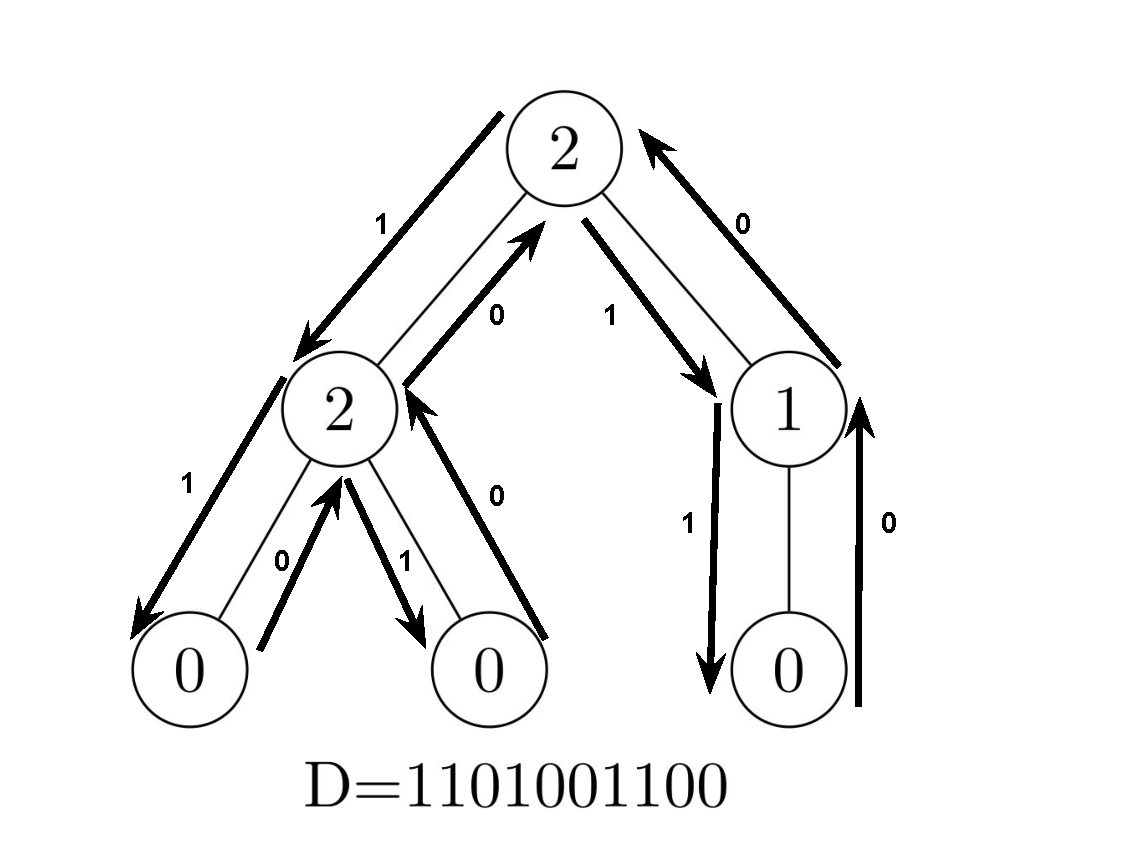
\includegraphics{Ordered-Tree-Bijection-Illustration}
    \caption{An ordered tree with $5+1=6$ nodes corresponding to the order 5 Dyck word $1101001100$.}
	\label{ordered_tree_bijection_illustration}
\end{figure}

%TODO: Combine the above and below figures?? Have them adjacent to each other?

\begin{figure}
$T=$

\begin{tikzpicture}[every tree node/.style={draw,circle},sibling distance=10pt, level distance=40pt]
\tikzset{edge from parent/.style={draw, edge from parent path=
    {(\tikzparentnode) -- (\tikzchildnode)}}}
    \Tree [.\node[style={fill=lightpurple}]{1}; [.\node[style={fill=lightpurple}]{G(2)}; [.\node[style={fill=lightpurple}]{P(3)};[.\node[style={fill=lightpurple}]{L(1)}; [.\node[style={fill=lightpurple}]{1}; [.\node[style={fill=lightpurple}]{1}; [.\node[style={fill=lightpurple}]{0}; ] ] ] ] [.O(1) [.0 ] ] [.0 ] ] [.1 [.0 ] ] ] ]
\end{tikzpicture}

$D=[1, 1, 1, 1, 1, 1, 0, 0, 0, 0, 1, 1, 0, 0, 1, 0, 0, 1, 1, 0, 0, 0]$
\caption{An ordered tree with 12 nodes corresponding to the Dyck word 1111110000110010011000.  Each node is labelled with its number of children; the left down path of T is highlighted in purple. Nodes are labelled by their degree.}
\label{exampleotree}
\end{figure}

Let $\otree{D}$ and $\dyck{T}$ be functions that convert a Dyck word to an ordered tree and an ordered tree to a Dyck word respectively via the above process. 


\subsubsection{Successor Rule}

Define the left-down path of an ordered tree T, denoted $\leftdown{T}$ to be the first $m+1$ nodes in a preorder traversal of T such that, for each $t_i$ with $0 \le i \le m$, $i=0$ or $t_i$ is the leftmost child of $t_{i-1}$.

Given an ordered tree T, let O be the first node in a preorder traversal of T that is not in the left-down path of T. If there is no such node, in the case where the tree is a single path, let O be the tree's (only) leaf node.  Let P be O's parent.  Let G be P's parent, and let L be P's leftmost child (or, equivalently, O's left sibling).  The labels P, G, and L are mnemonics for O's (p)arent, (g)randparent, and (l)eft sibling. 
 Fig. \ref{exampleotree} gives an example illustrating O,P,G,L, and the left-down path in an tree.


The successor rule for enumerating ordered trees with n nodes can be stated as folows:

\begin{subnumcases}{\nextTree{T} = \label{eq:otreeRule}}
    \treeshift{T}{O}{root} & $\leftdown{T}=T$ \label{eq:otree_noo}\\
    \treeshift{\treeshift{T}{L}{G}}{O}{root}& if $P \ne root $ and O has no children \label{eq:otree_zeroshift}\\
    \treeshift{T}{L}{O} & otherwise \label{eq:otree_oneshift}
\end{subnumcases}
% \footnote{important: 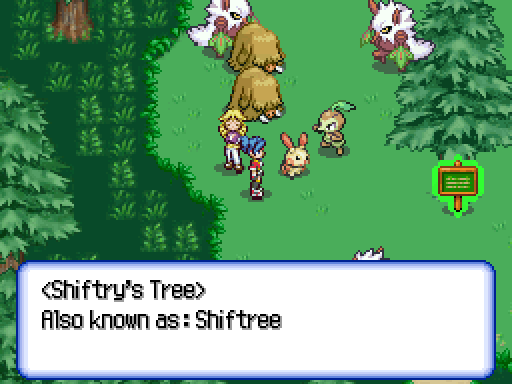
\includegraphics[width=.3\textwidth]{shiftree}} 

\subsubsection{Proof of Correctness} -- still somewhat of an outline.


HELPFUL FUNCTIONS 

$\depth{t_i}=$ length of path between root and $t_i$. $\depth{root}=0$

$\ithone{D}{i}=$ the index of the $i\thh{}$ one in D.

Let $\dyckindex{N}$ be a function that converts a ordered tree node n to the index of its corresponding $1$ in $\dyck{T}$. Similarly,% $\zeroesbetween{D}{i}{j}=$ the number of zeroes between the $i$th and $j$th 

\bigskip

HELPFUL LEMMAS
\begin{enumerate}
    \item $t_i$ corresponds to the $i$th one in D for $1 \le i \le n$
	This is due to the nature of the bijection between Dyck words and ordered trees.  Each one in D creates a new node; zeroes in D do not create nodes.  Generating an ordered tree from a Dyck word generates the nodes of the tree in preorder.  Thus, $t_i$ corresponds to the $i$th one in D for $1 \le i \le n$.
    \item $\depth{t_i}=\depth{t_{i-1}}+1-(\ithone{D}{i}-\ithone{D}{i-1}-1)$ \\
	Note that $(\ithone{D}{i}-\ithone{D}{i-1}-1)$ is equal to the number of zeroes between the $i\thh$ and $(i-1)^{\underline{st}}$ ones in D.  


	Informally, depth of $t_i$ is the depth of $t_{i-1}$ plus 1 minus the number of zeroes between $t_{i-1}$ and $t_{i}$

	This also follows naturally from the bijection between Dyck words and ordered trees.  Each zero corresponds to a step up in the tree before adding the next child.  

	If there are zero zeroes between the $i\thh$  and $(i-1)^{\underline{st}}$ ones in D, $t_i$ is a child of $t_{i-1}$; $\depth{t_i}=\depth{t_{i-1}}+1$

	If there is one zero between the $i\thh$  and $(i-1)^{\underline{st}}$ ones in D, $t_i$ is a child of $t_{i-1}$'s parent; $\depth{t_i}=\depth{t_{i-1}}+1$.  

	Each subsequent zero between $t_{i-1}$ and $t_i$ decreases $\depth{t_{i}}$ by one.  Thus, the depth of $t_i$ is the depth of $t_{i-1}$ plus 1 minus the number of zeroes between $t_{i-1}$ and $t_{i}$.



    \item $\depth{O}=m-j+1$

	$t_m$ is the last node in the $\leftdown{T}$, as the left-down path has m+1 nodes. It has depth m, as it is exactly m left-down steps from the root.  Note that $O=t_{m+1}$.  The number of zeroes between $t_m$ and $t_{m+1}$ is the number of zeroes between the $m\thh$ and $(m+1)^{\underline{st}}$ ones in $D_i$.  

    \item Preorder listing of T $\implies $ D

	Let $T=t_0,t_1,...t_n$ be a preorder traversal of T.  Note that $t_0$ is the root of $T$

	Construct D as follows: 

	\begin{itemize}
 	\item skip $t_0$
	    \item Let $D=\epsilon$ % clear that this is empty string?
	\item For each $t_i$, $1\le i \le n$
	\begin{itemize}
 	\item Append a 1 to $D$
	\item Append $1-\depth{t_{i-1}}+\depth{t_{i}}$ zeroes to D.
 \end{itemize}
 \end{itemize}
 \item Every non-leaf node below P in $\leftdown{T}$ has exactly 1 child.  

     If a node below P in $\leftdown{T}$ had a second child, that child would not be in $\leftdown{T}$ and would be be traversed before O in preorder, which would be a contradiction. 


\end{enumerate}

Ruskey and Williams proved that, given a Dyck word of order n, \ref{eq:prefixDyck} iteratively generates all Dyck words of order n.  This proof will use the bijection between Dyck words of order $n$ and ordered trees with $n+1$ nodes to show that that \ref{eq:otreeRule} generates all ordered trees with a given number of nodes.  

To prove that $\nextTree{T}$ generates all ordered trees with $|T|$ nodes, it is sufficient to show that, given a Dyck word D and its corresponding ordered tree T, 

$\coolCat{D}=\dyck{\nextTree{T}}$

\bigskip


In other words, we aim to show that $\coolCat{D}=\dyck{\nextTree{\otree{D}}}$


First, consider the node O in the specification of the $\nextTree{T}$ algorithm.  

Let $D=\dyck{T}$ and let k be the index of the 1 in the leftmost 01 substring of D.  Let $t_0...t_m=\leftdown{T}$; $O=t_{m+1}$.  We will show that O corresponds to $D_k$.

(This can be done better) 

Note that each 1 in D corresponds to a step down; each 0 to a step up.  Consequently, $\leftdown{T}$ corresponds to the ``all-one" prefix of D.  In other words, $\leftdown{T}=t_0,t_1,...t_{m}$ such that $i=0$ or $D_{\dyckindex{t_i}}=1$. Note that $t_{m+1}$ is therefore the first node in a preorder traversal of T such that $D_{\ithone{D}{m+1}}=1$ and $D_{\ithone{D}{m+1}-1}=0$ and the first node in a preorder traversal of T such that $t_m \notin \leftdown{T}$.  Therfore, $\ithone{D}{m+1}=k$, i.e., $t_{m+1}=O$ corresponds to the 1 in the leftmost 01 substring of D.



$\coolCat{D}$ and $\nextTree{T}$ are each broken down into 3 cases in equations \ref{eq:prefixDyck} and \ref{eq:otreeRule} respectively. 

\begin{subnumcases}{\coolCat{D} = \label{eq:expandedDyck}}
    \preshift{D}{2n} & \text{if $D$ has no $01$ substring} \label{eq:expandedDyck_n}\\
	\preshift{D}{k+1} & $D_{k+1}=1$ \label{eq:expandedDyck_k1_1}\\
	\preshift{D}{k+1} & $D_{k+1}=0$ and $m>\frac{k-1}{2}$ \label{eq:expandedDyck_k1_0}\\
	\preshift{D}{k} & $D_{k+1}=0$ and $m=\frac{k-1}{2}$ \label{eq:expandedDyck_k}
\end{subnumcases}

\begin{subnumcases}{\nextTree{T} = \label{eq:expandedOtree}}
    \treeshift{T}{O}{root} & $\leftdown{T}=T$ \label{eq:ex_otree_n}\\
    \treeshift{T}{L}{O} & if O has at least 1 child \label{eq:ex_otree_k1_1} \\
    \treeshift{\treeshift{T}{L}{G}}{O}{root}& if $P \ne root $ and O has no children \label{eq:ex_otree_k1_0} \\
    \treeshift{T}{L}{O} & if O has no children and $P=root$ \label{eq:ex_otree_k}
\end{subnumcases}

% \footnote{important: 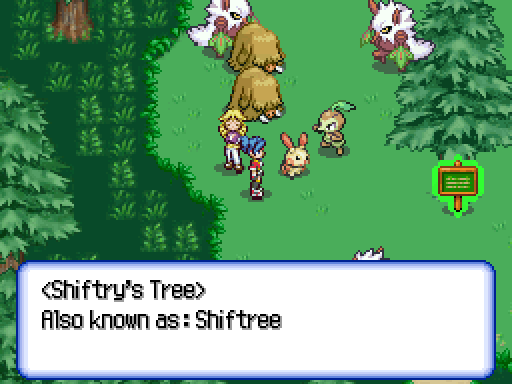
\includegraphics[width=.3\textwidth]{shiftree}} 

For convenience, equations \ref{eq:expandedDyck} and \ref{eq:expandedOtree} give the expanded restatemtents of the successor rules for $\coolCat{D}$ and $\nextTree{T}$ that to facilitate comparisons between the two.  

We will show the following equivalences:

TODO: use the cases from 5, make this easier
\begin{enumerate}
    \item \ref{eq:otree_noo} corresponds to \ref{eq:prefixDyck_n}
    \item \ref{eq:otree_zeroshift} corresponds to \ref{eq:expandedDyck_k1_0}
	% \begin{itemize}
 	% \item Case equivalence: $D_{k+1}=0$ and $D$ starts with more than $\lfloor \frac{k-1}{2} \rfloor$ ones \iff $O$ is not the child of the root or
 % \end{itemize}
    \item \ref{eq:otree_oneshift} corresponds to \ref{eq:expandedDyck_k1_1} and \ref{eq:expandedDyck_k}
\end{enumerate}

To show these, first we show a few auxillary equivalences:

Let $m$ be the number of consecutive ones to start D, let $j$ be the number of consecutive zeroes starting at $d_{m+1}$.  Note that $j=(k-m-1)$; $d_{k}=1$
\begin{itemize}
    \item $D$ has no 01 substring $\iff$ $LD(T)=T$


	If $D$ has no $01$ substring, $D=1^n0^n$, and T is $n+1$ nodes where $t_0$ is the root and each $t_i$ for $1\le i \le n$ is a child of $t_{i-1}$  In this case, $T$ is essentially a path of $n+1$ nodes, and the left-down path of T is the entire tree.
    \item $D_{k+1} = 0 \iff O$ has no children

	This follows logically from the bijection between Dyck words and ordered trees.  $D_k$ corresponds to O.  If $D_{k+1}=0$, an ``upward" step is taken after O and consequently the next node after O cannot be a child of O.  Since the ones in $D$ give the nodes of T in preorder, O must have no children.

	Informally, once you go ``up" from O, the bijection between Dyck words and ordered trees gives no way to go ``back down" to give O an additional child.
    \item $P=root \iff D$ starts with exactly $\frac{k-1}{2}$ ones.

	First, note that $P=root$ simply means that O is a child of the root.

	Next, note that the number of nodes in $\leftdown{T}$ is equal to the number of consecutive ones at the start of $D$.  Let $m$ be the number of consecutive ones at the start of $D$.  Note that $k-m-1$ is the number of consecutive zeroes following $d_m$, since $d_k$ is the index of the 1 in the first 01 substring of D. Since each of the $m$ ones constitutes a step down from the root in $T$ and each of the $k-m-1$ zeroes starting at $d_m$ corresponds a step up towards the root in T, $m=k-m-1 \iff $ O is a child of the root. 

	This equivalence can can be rewriten as follows: 

	$m=k-m-1$

	$2m=k-1$

	$m=\frac{k-1}{2}$


	Therefore, $P=root \iff D$  starts with $\frac{k-1}{2}$ ones.

    \item $L$ corresponds to $D_{m-j+1}$

	
\end{itemize}
\begin{enumerate}
    \item \ref{eq:otree_noo} corresponds to \ref{eq:expandedDyck_n}

	\begin{itemize}
	    \item It was previously shown that $D$ has no 01 substring $\iff$ $LD(T)=T$.  

		Thus, $\nextTree{T}$ executes case \ref{eq:otree_noo} if and only if $\coolCat{D}$ executes case  \ref{eq:expandedDyck_n}

		TODO: show the shifts are equivalent.
	\end{itemize}
    \item \ref{eq:otree_zeroshift} corresponds to \ref{eq:expandedDyck_k1_0}

	\begin{itemize}
	    \item It was previously shown that $P=root \iff D$ starts with exactly $\frac{k-1}{2}$ ones.  

		It was also previously shown that $D_{k+1}=0 \iff O$ has no children.  
		Thus, $\nextTree{T}$ executes case \ref{eq:otree_zeroshift} 
		if and only if $\coolCat{D}$ executes case   \ref{eq:expandedDyck_k1_0}

	    \item We now show that the execution of \ref{eq:otree_zeroshift} is equivalent to the execution of    \ref{eq:expandedDyck_k1_0}.

		Given $\dyck{T}=D=1^m0^{j}10d_{k+2}d_{k+3}...d_{2n}$, we aim to show that 

		$\dyck{\nextTree{T}}=\coolCat{\dyck{T}}$
\bigskip
\bigskip

		Note that $\nextTree{T}=\treeshift{\treeshift{T}{L}{G}}{O}{root}$. 




		Let $T'=\treeshift{T}{L}{G}$; $T''=\treeshift{T'}{O}{root}$

		Note that $\nextTree{T}=T''$

		Since $P \ne root$, we know that G, the parent of P, exists. 
		Thus, we can assume that $G,P,L \in \leftdown{T}$.  Furthermore, recall that L (and all other non-leaf nodes $\in \leftdown{T}$ must have exactly one child.  Therefore, every node below L in $\leftdown{T}$ has its depth reduced by one; no other nodes have their depth affected by this shift.


		% this should be a little lemma
		% $T'$ shifts T so that L becomes the first child of G.  Note that L must have exactly 1 child: otherwise L's second child would be traversed earlier in a preorder traversal than O.  The same logic holds for each subtree of L: Each of L's non-leaf descendents must have exactly one child, as otherwise O would not be the first node in a preorder traversal of T not in $\leftdown{T}$.

		\bigskip
		\bigskip

		$T=$
		\begin{center}
		\begin{tabular}{ |c|c|c|c|c|c|c|c|c|c|c| } 
		 \hline

		    $node$ & $t_0$ & $t_1$ & $\dots$ & $G=t_{m-j-1}$ & $P=t_{m-j}$ & $L=t_{m-j+1}$ & $\dots$ & $t_m$ & $O=t_{m+1}$ & $\dots$ \\
		 \hline
		 $depth$ & $0$ & $1$ & $\dots$ & $(m-j-1)$ & $(m-j)$ & $(m-j+1)$ & $\dots$ & $m$  & $(m-j+1)$ & $\dots$\\
		 \hline
		    $Dyck$ &  &  \multicolumn{7}{|c|}{$1^m$} &  $0^{j}1$   & $0\dots$\\
		 \hline
		\end{tabular}
		\end{center}


		\bigskip
		\bigskip


		$T'=$
		\begin{center}
		\begin{tabular}{ |c|c|c|c|c|c|c|c|c|c|c| } 
		 \hline

		    $node$ & $t_0$ & $t_1$ & $\dots$ & $G=t_{m-j-1}$ & $L=t_{m-j+1}$ & $\dots$ & $t_m$ & $P=t_{m-j}$ & $O=t_{m+1}$ & $\dots$ \\
		 \hline
		 $depth$ & $0$ & $1$ & $\dots$ & $(m-j-1)$ & $(m-j)$ & $\dots$ & $m-1$ & $(m-j)$  & $(m-j+1)$ & $\dots$\\
		 \hline
		    $Dyck$ &  &  \multicolumn{6}{|c|}{$1^{m-1}$} &  $0^{j}1$   & $1$ & $0\dots$\\
		 \hline
		\end{tabular}
		\end{center}

		This operation makes P G's second child, consequently removing P from the left-down path of $T'$ and making P the first node in a preorder traversal of $T'$ that is not in the left-down path of $T'$.  Therefore, $|\leftdown{T'}|=m-1$; $O'=P$. 

		Note in the case where $j=1$, $L=t_m$; i.e. L is the leaf of the left-down path of T.

		Recovering a Dyck word from $T'$, we obtain 

		D'=$1^{m-1}0^j110d_{k+1}d_{k+3},\dots,d_{2n}$


		Next, we use $\treeshift{T'}{O}{root}$ to obtain $T'' = \nextTree{T}$

$\treeshift{T'}{O}{root}$ shifts O to become the first child of the root. Note that we know that O has no children. Consequently, no nodes other than O have their depth affected by this shift. Thus, 

\bigskip
\bigskip


		% TODO: tm+2 dots, here and other tables
		$T''=$
		\begin{center}
		\begin{tabular}{ |c|c|c|c|c|c|c|c|c|c|c|c| } 
		 \hline

		    $node$ & $t_0$ & $O=t_{m+1}$ & $t_1$ & $t_2$ & $\dots$ & $G=t_{m-j-1}$ & $L=t_{m-j+1}$ & $\dots$ & $t_m$ & $P=t_{m-j}$ & $\dots$ \\
		 \hline
		    $depth$ & $0$ & $1$ & $1$ & $2$ &$\dots$ & $(m-j-1)$ & $(m-j)$ & $\dots$ & $m-1$ & $(m-j)$   & $\dots$\\
		 \hline
		    $Dyck$ &  & $1$ &  \multicolumn{7}{|c|}{$01^{m-1}$} &  $0^{j}1$   & $\dots$\\
		 \hline
		\end{tabular}
		\end{center}


		% Next, recovering a Dyck word from $$
		\bigskip
		\bigskip

		% TODO: refine



		Therefore, since $T''=\nextTree{T}$, $\dyck{\nextTree{T}}=101^{m-1}0^j1\dots$

		Since $\dyck{T}=D=1^m0^{j}10\dots$
		$\ref{eq:expandedDyck_k1_1}$ gives that

		$\coolCat{\dyck{T}}=101^{m-1}0^j1\dots$

		Therefore, we have shown that $\dyck{\nextTree{T}}=\coolCat{\dyck{T}}=101^{m-1}0^j1\dots$
	\end{itemize}

    \item \ref{eq:otree_oneshift} corresponds to \ref{eq:expandedDyck_k1_1} and \ref{eq:expandedDyck_k}

	``otherwise" in case \ref{eq:otree_oneshift} corresponds to the following:
	\begin{itemize}
	    \item At least 1 node in T is not in $\leftdown{T}$ and (O has at least 1 child OR (O has no children and O is a child of the root))
	\end{itemize}

	Combining cases \ref{eq:expandedDyck_k1_1} and \ref{eq:expandedDyck_k} gives the following condition:
	\begin{itemize}
	    \item D has a 01 substring and ($D_{k+1}=1$ OR ($D_{k+1}=0$ and D starts with exactly $\frac{k-1}{2}$ ones))

	\end{itemize}

	These are equivalent. 

	$T \ne \leftdown{T} \iff D$ has a 01 substring.

	$D_{k+1}=1 \iff O$ has at least one child.

	$D_{k+1}=0$ and $m=\frac{k-1}{2} \iff O$ has no children and O is a child of the root.

	TODO: elaborate. Thus, \ref{eq:otreeRule} executes case \ref{eq:otree_zeroshift} if  $\coolCat{D}$ executes case \ref{eq:expandedDyck_k1_1}

	Execution equivalence: 

	Given the above,

	\begin{itemize}
	    \item Given D has a 01 substring $\iff \leftdown(T) \ne T$ and 

		$D_{k+1}=1 \iff$ $O$ has at least one child
\bigskip

		\ref{eq:expandedDyck_k1_1} corresponds to  \ref{eq:otree_oneshift}

	    $\preshift{\dyck{T}}{k+1}=\treeshift{T}{L}{O}$

		$D=1^m0^j11$


		$T=$
		\begin{center}
		\begin{tabular}{ |c|c|c|c|c|c|c|c|c|c|c|c| } 
		 \hline

		    $node$ & $t_0$ & $t_1$ & $\dots$ & $G=t_{m-j-1}$ & $P=t_{m-j}$ & $L=t_{m-j+1}$ & $\dots$ & $t_m$ & $O=t_{m+1}$ & $t_{m+2}\dots$ \\
		 \hline
		    $depth$ & $0$ & $1$ & $\dots$ & $(m-j-1)$ & $(m-j)$ & $(m-j+1)$ & $\dots$ & $m$  & $(m-j+1)$ & $m-j+2 \dots$\\
		 \hline
		    $Dyck$ &  &  \multicolumn{7}{|c|}{$1^m$} &  $0^{j}1$   & $1\dots$\\
		 \hline
		\end{tabular}
		\end{center}

		Shift L to be O's first child: L:$t_m$ come after O in preorder traversal, 
	%%%%%%%%%%%%%%%%%%%%%%%%%%%
	\item Given D has a 01 substring, and $D_{k+1}=0$ and $D$ starts with exactly $\frac{k-1}{2}$ ones 

	    \ref{eq:expandedDyck_k} corresponds to  \ref{eq:otree_oneshift}

	    $\preshift{\dyck{T}}{k}=\treeshift{T}{L}{O}$
	    Case equivalence: 


     \end{itemize}
\end{enumerate}



\subsubsection{Loopless Implementation}
todo
